%==============================================================================
% 6 RESULTS I: IDENTIFIABILITY BY EXCITATION REGIME
% Plano: modelo identificado (Tab.) e o ajuste de yaw em malha fechada (K 1.378, fit
% 44.8 %); diluicao (1 % da atuacao por roda, 56 % da variancia); C1 (gerador linear
% recupera theta* sempre que ha excitacao; fit % mede SNR); C1b (gerador fisico
% reproduz a inflacao +16.5 / +27.4 %, controle sem translacao 0.988 / 0.930,
% rotacao dedicada 0.996): Fig. e Tab.
% Fontes: tab_journal_identified, tab_journal_insilico_yaw, fig_journal_identifiability
% (geradas); CHANGELOG 2026-09-07 15:52 (C1) e 20:45 (C1b v2).
%==============================================================================
\section{Results I: identifiability follows the excitation regime}
\label{sec:res-ident}

% ==============================================================================
% tab_journal_identified: generated by `dtssl analysis run journal_tables` (dtssl.analysis.journal_tables).
% Do not edit by hand: re-run the generator. Sources:
%   config/twin_params.json (K, tau, Td)
%   results/CHANGELOG.md 2026-06-14 10:24 and 2026-07-24 17:35 (hold-out fits)
%   results/loo_translational_20260810_1743.md
%   results/r3_closedloop_omega_fit_20260810_1036.md
% ==============================================================================
% Needs \usepackage{booktabs,adjustbox}.
\begin{table*}[t]
\centering
\caption{Identified per-DOF first-order-plus-dead-time parameters and hold-out fit (Eq. fit). The yaw channel fitted on closed-loop competition logs is shown for contrast; it fails the 60\% gate and is not promoted.}
\label{tab:identified}
\small
\begin{adjustbox}{max width=\textwidth}
\begin{tabular}{lccccll}
\toprule
DOF & $K$ & $\tau$ (s) & $T_d$ (s) & hold-out fit (\%) & data & leave-one-event-out fit (\%) (folds) \\
\midrule
$v_x$ & 1.119 & 0.072 & 0.069 & 86.7 & competition, \texttt{front\_to\_back} & $84.3\pm2.0$ (4) \\
$v_y$ & 1.052 & 0.127 & 0.056 & 87.1 & competition, \texttt{side\_to\_side} & $82.8\pm2.7$ (13) \\
$\omega$ & 1.002 & 0.083 & 0.089 & 71.1 & dedicated open-loop rotation & -- \\
\midrule
$\omega$, closed loop (not promoted) & 1.378 & 0.043 & 0.112 & 44.8 & competition, \texttt{shoot\_to\_goal} & -- \\
\bottomrule
\end{tabular}
\end{adjustbox}
\end{table*}


\begin{figure*}[t]
  \centering
  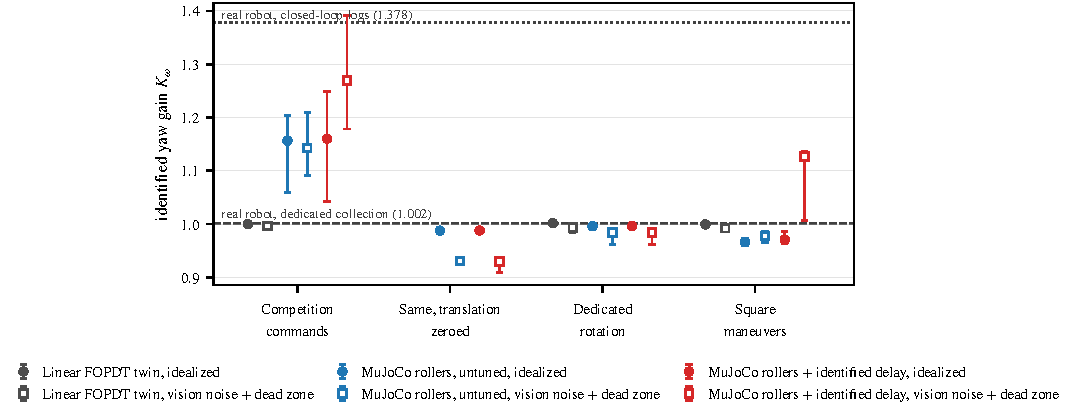
\includegraphics[width=0.74\textwidth]{fig_journal_identifiability.pdf}
  \caption{Yaw gain re-identified from synthetic logs generated by a known plant, by excitation regime. Markers: median over replicates; bars: interquartile range. Horizontal lines: the real robot's estimates from closed-loop competition logs and from the dedicated open-loop collection.}
  \label{fig:ident}
\end{figure*}

% ==============================================================================
% tab_journal_insilico_yaw: generated by `dtssl analysis run journal_tables` (dtssl.analysis.journal_tables).
% Do not edit by hand: re-run the generator. Sources:
%   results/identifiability_insilico_20260907_1552.json
%   results/identifiability_insilico_mujoco-rollers_v2_20260907_2048.json
%   results/identifiability_insilico_mujoco-rollers-delay_v2_20260907_2044.json
%   results/r3_closedloop_omega_fit_20260810_1036.md
%   config/twin_params.json (K_w = 1.0016)
% ==============================================================================
% Needs \usepackage{booktabs,adjustbox}.
\begin{table*}[t]
\centering
\caption{Yaw gain re-identified from synthetic logs generated with a known plant, by excitation regime and generator.}
\label{tab:insilico-yaw}
\small
\begin{adjustbox}{max width=\textwidth}
\begin{tabular}{lcccccc}
\toprule
& \multicolumn{2}{c}{linear FOPDT twin} & \multicolumn{2}{c}{MuJoCo rollers} & \multicolumn{2}{c}{MuJoCo rollers + delay} \\
\cmidrule(lr){2-3} \cmidrule(lr){4-5} \cmidrule(lr){6-7}
regime & idealized & noise + dead zone & idealized & noise + dead zone & idealized & noise + dead zone \\
\midrule
competition commands & 1.000 [1.000, 1.000] & 0.996 [0.996, 0.997] & 1.156 [1.059, 1.204] & 1.143 [1.092, 1.209] & 1.160 [1.043, 1.249] & 1.270 [1.179, 1.391] \\
same, translation zeroed & -- & -- & 0.988 [0.986, 0.989] & 0.931 [0.926, 0.936] & 0.988 [0.987, 0.989] & 0.930 [0.910, 0.937] \\
dedicated rotation & 1.002 [1.002, 1.002] & 0.994 [0.985, 0.995] & 0.996 [0.996, 0.996] & 0.984 [0.962, 0.988] & 0.996 [0.996, 0.996] & 0.984 [0.962, 0.988] \\
square maneuvers & 0.999 [0.999, 1.000] & 0.992 [0.988, 0.995] & 0.967 [0.960, 0.973] & 0.977 [0.966, 0.986] & 0.971 [0.963, 0.987] & 1.127 [1.007, 1.137] \\
designed excitation & 1.001 [1.001, 1.001] & 1.000 [0.999, 1.000] & 1.015 [0.965, 1.057] & 1.065 [1.015, 1.113] & 1.031 [0.981, 1.060] & 0.986 [0.950, 1.021] \\
\bottomrule
\end{tabular}
\end{adjustbox}

\vspace{2pt}
\parbox{\linewidth}{\footnotesize Median [25th, 75th percentile] over replicates (20 for the linear twin, 12 for MuJoCo). Idealized: no measurement noise, dead zone off; noise + dead zone: vision noise of 2 mm and 0.01 rad with the firmware per-wheel dead zone. Designed excitation: R3 for the linear twin, the milder R3-mild inside the traction envelope of the rollers model for MuJoCo. Real robot: 1.378 from closed-loop logs, 1.002 from the dedicated collection.}
\end{table*}


\pending{text of the section.}
